\chapter{移动平台设计和制造}
\label{cha:Platform}

\section{平台设计初始思路}
形式:

每个小车为一个数据点,在1-3维坐标系内动态运动(如果和ShapeBots\cite{suzuki2019shapebots}一样具备升降平台或者和SwarmOS一样具备可变色LED点阵则可以进行三维变量显示)

也可以每个小车作为一个通信节点(在电力市场的应用场景下是一个机组节点),用屏幕/位置/RGB颜色/高度直观的显示迭代的过程。

即插即用的实现:放入/取出小车,新的迭代随即开始。

\section{仿真}

Swarm仿真参考ShapeBots\cite{suzuki2019shapebots}的仿真方法\footnote{\href{https://ryosuzuki.github.io/shapebots-simulator/}{https://ryosuzuki.github.io/shapebots-simulator/}},使用Javascript在网页端编写了相应的仿真程序,进行指定数量的集群小车对于SVG格式图片的渲染和给定数据折线图或条形图的可视化绘制。

\section{定位方法}

% 如果直接插入一页PDF用
% 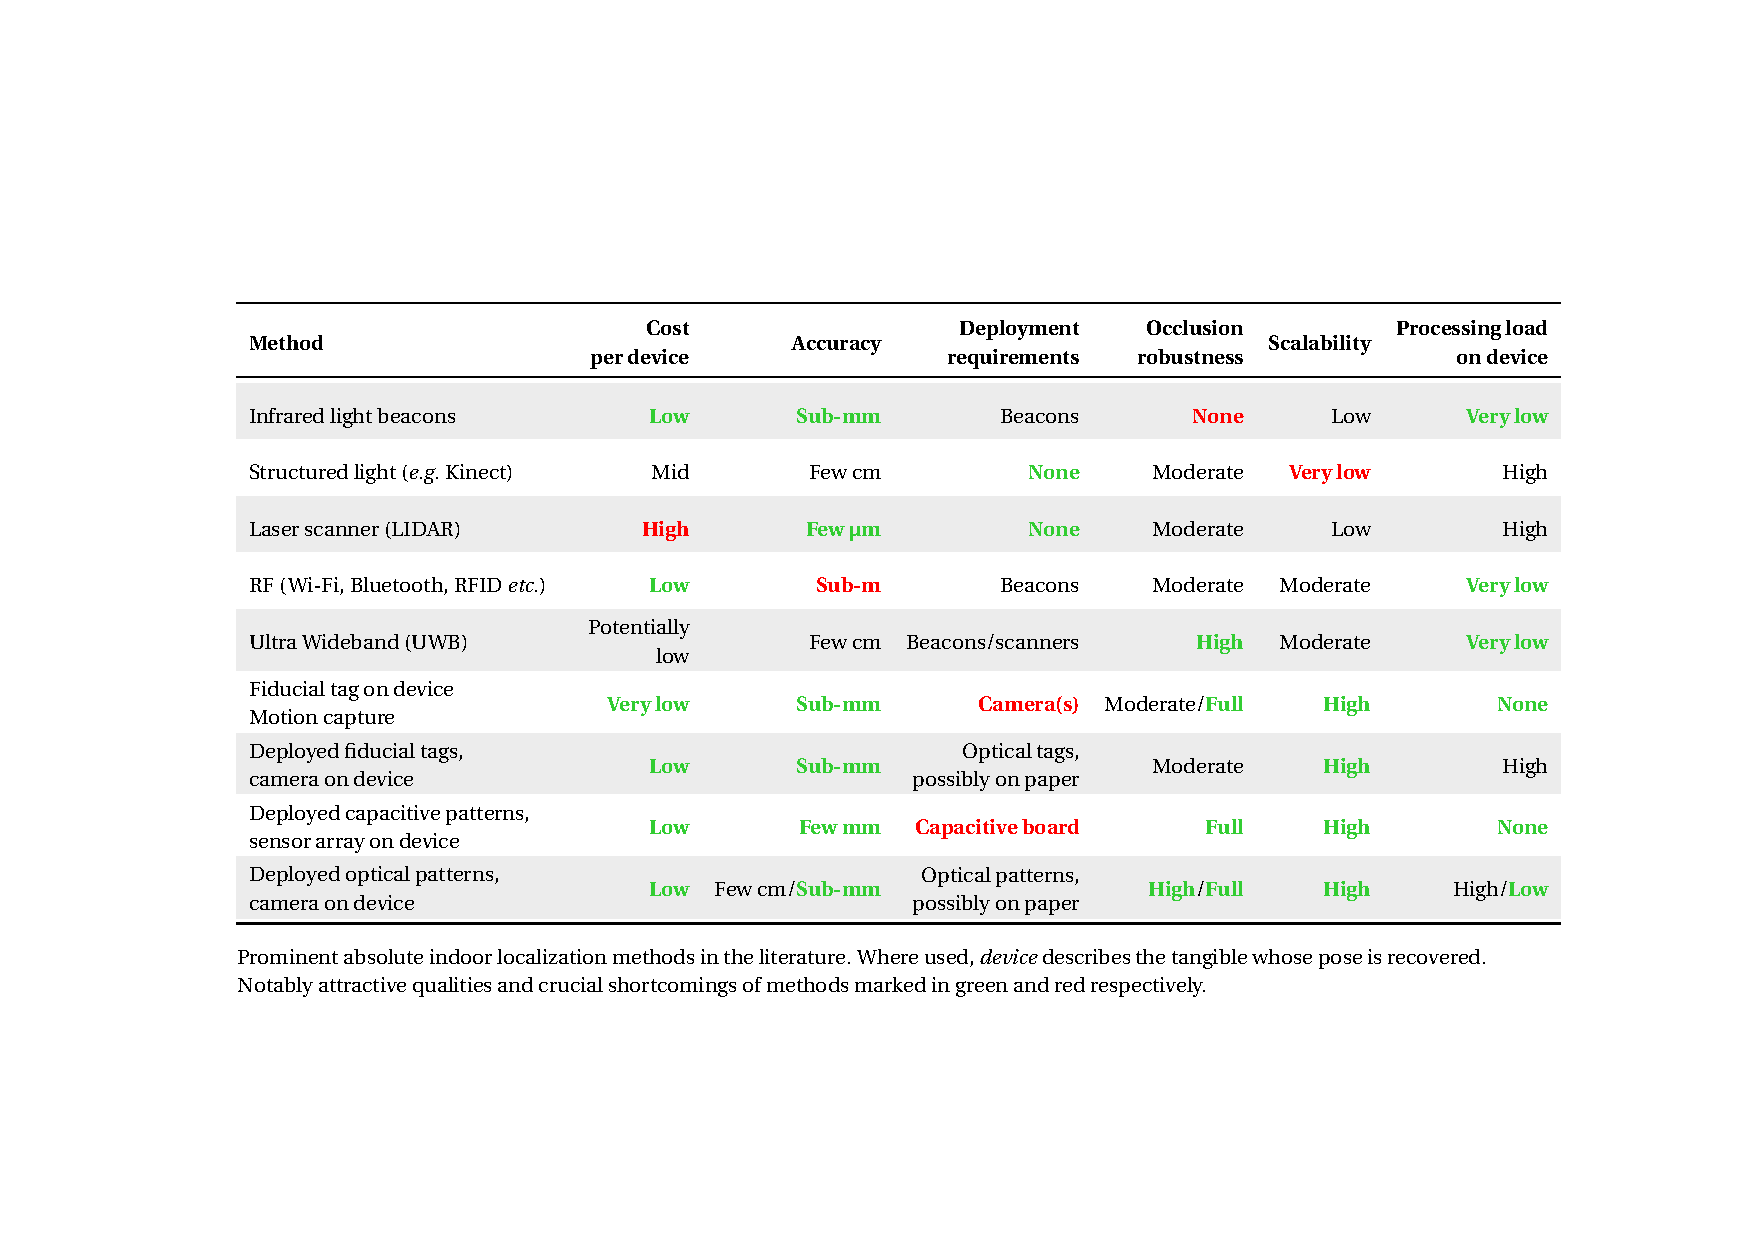
\includepdf{Prominent-absolute-indoor-localization-methods-comparison.pdf} 

% Please add the following required packages to your document preamble:
% \usepackage[table,xcdraw]{xcolor}
% If you use beamer only pass "xcolor=table" option, i.e. \documentclass[xcolor=table]{beamer}
% \usepackage{lscape}
\begin{landscape}
    \begin{table}[]
    \centering
    \begin{tabular}{lllllll}
    \hline
    Method                                                                                         & Cost per device & Accuracy      & \begin{tabular}[c]{@{}l@{}}Deployment\\ requirements\end{tabular}             & \begin{tabular}[c]{@{}l@{}}Occlusion\\ robustness\end{tabular} & Scalabiity & \begin{tabular}[c]{@{}l@{}}Processing load\\ on device\end{tabular} \\ \hline
    \rowcolor[HTML]{EFEFEF} 
    Infrared light beacons                                                                         & Low             & Sub-mm        & Beacons                                                                       & None                                                           & Low        & Very low                                                            \\
    Structured light (e.g. Kinect)                                                                 & Mid             & Few cm        & None                                                                          & Moderate                                                       & Very low   & High                                                                \\
    \rowcolor[HTML]{EFEFEF} 
    Laser scanner (LIDAR)                                                                          & High            & Few µm        & None                                                                          & Moderate                                                       & Low        & High                                                                \\
    \begin{tabular}[c]{@{}l@{}}RF (Wi-Fi, \\ Bluetooth, RFID etc.)\end{tabular}                    & Low             & Sub-m         & Beacons                                                                       & Moderate                                                       & Moderate   & Very low                                                            \\
    \rowcolor[HTML]{EFEFEF} 
    \begin{tabular}[c]{@{}l@{}}Ultra Wideband \\ (UWB)\end{tabular}                                & Potentially low & Few cm        & Beacons/scanners                                                              & High                                                           & Moderate   & Very low                                                            \\
    \begin{tabular}[c]{@{}l@{}}Fiducial tag on device\\ Motion capture\end{tabular}                & Very low        & Sub-mm        & Camera(s)                                                                     & Moderate/Full                                                  & High       & None                                                                \\
    \rowcolor[HTML]{EFEFEF} 
    \begin{tabular}[c]{@{}l@{}}Deployed fiducial tags,\\ camera on device\end{tabular}             & Low             & Sub-mm        & \begin{tabular}[c]{@{}l@{}}Optical tags, \\ possibly on paper\end{tabular}    & Moderate                                                       & High       & High                                                                \\
    \begin{tabular}[c]{@{}l@{}}Deployed capacitive patterns,\\ sensor array on device\end{tabular} & Low             & Few mm        & Capacitive board                                                              & Full                                                           & High       & None                                                                \\
    \rowcolor[HTML]{EFEFEF} 
    \begin{tabular}[c]{@{}l@{}}Deployed optical patterns,\\ camera on device\end{tabular}          & Low             & Few cm/Sub-mm & \begin{tabular}[c]{@{}l@{}}Optical patterns,\\ possibly on paper\end{tabular} & High/Full                                                      & High       & High/Low                                                            \\ \hline
    \end{tabular}
    \caption{Prominent absolute indoor localization methods in the literature. Where used, device describes the tangible whose pose is recovered. }
    \label{tab:localization}
    \end{table}
\end{landscape}

各类定位方法优缺点\cite{ozgur2018cellulo}如表~\ref{tab:localization}所示。

\section{底盘}
考虑到交互过程中需要推动小车,通过用户调查我们知道:大多数用户(特别是儿童)习惯于按压着移动小车,这就使得我们不能采用Zooids\cite{le2016zooids}(如图~\ref{fig:Zooids})或e-puck\cite{mondada2009puck}(如图~\ref{fig:e-puck})使用的差速转向,只能采用类似Cellulo\cite{ozgur2017cellulo}(如图~\ref{fig:Cellulo})的磁驱技术或WolfBot\cite{betthauser2014wolfbot}(如图~\ref{fig:WolfBot})使用的全向轮。

\begin{figure}[htbp]
    \centering
    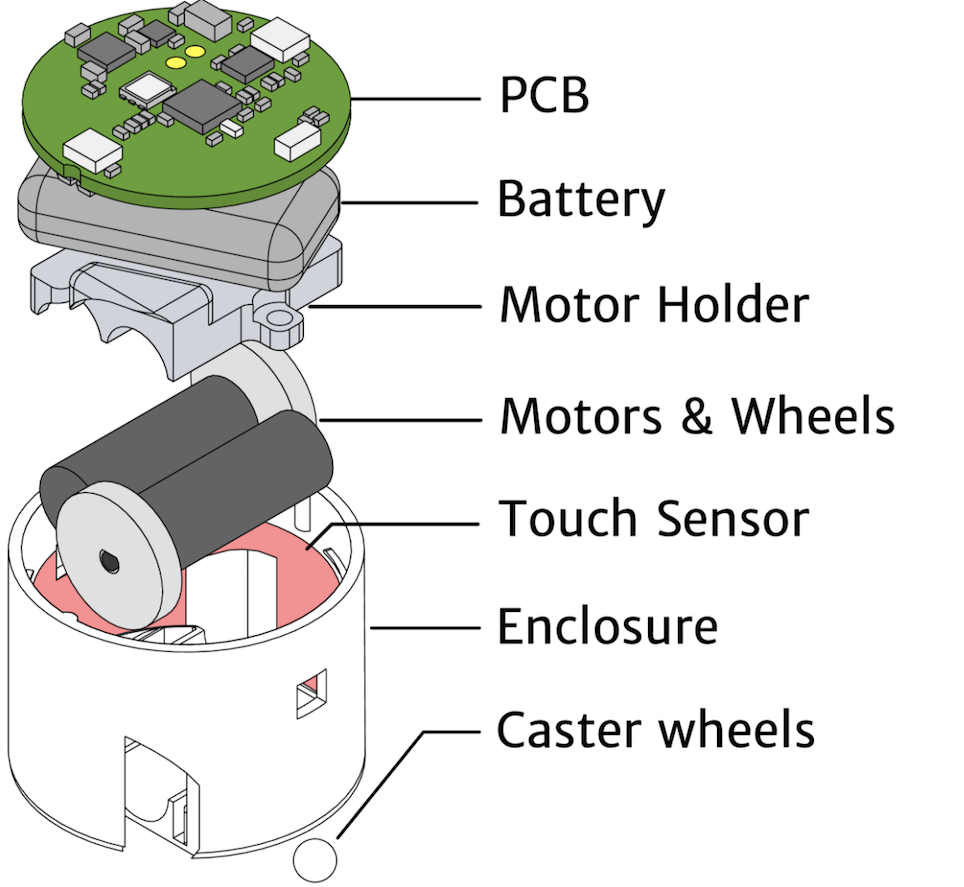
\includegraphics[height=10cm]{Zooids.png}
    \caption{Zooids}
    \label{fig:Zooids}
\end{figure}

\begin{figure}[htbp]
    \centering
    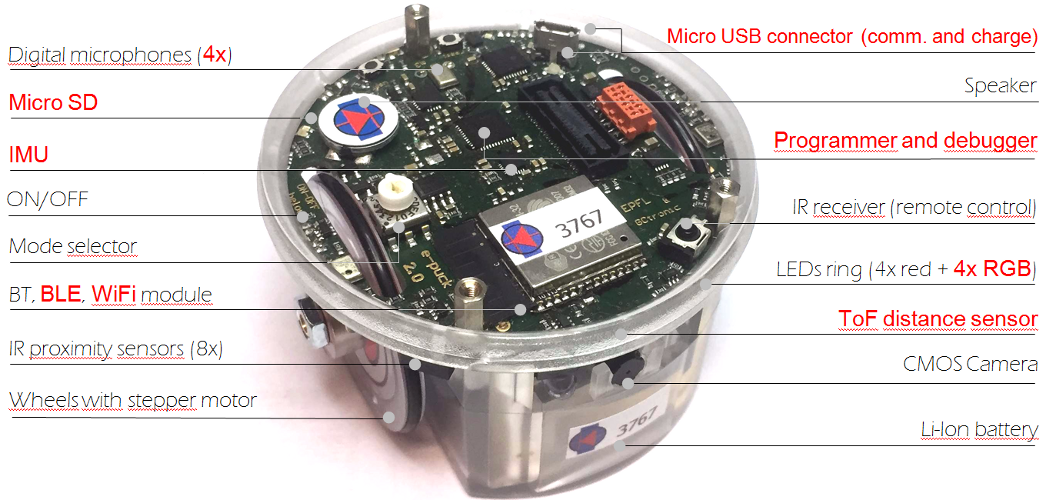
\includegraphics[height=6cm]{e-puck2-features_small.png}
    \caption{Zooids}
    \label{fig:e-puck}
\end{figure}

\begin{figure}[htbp]
    \centering
    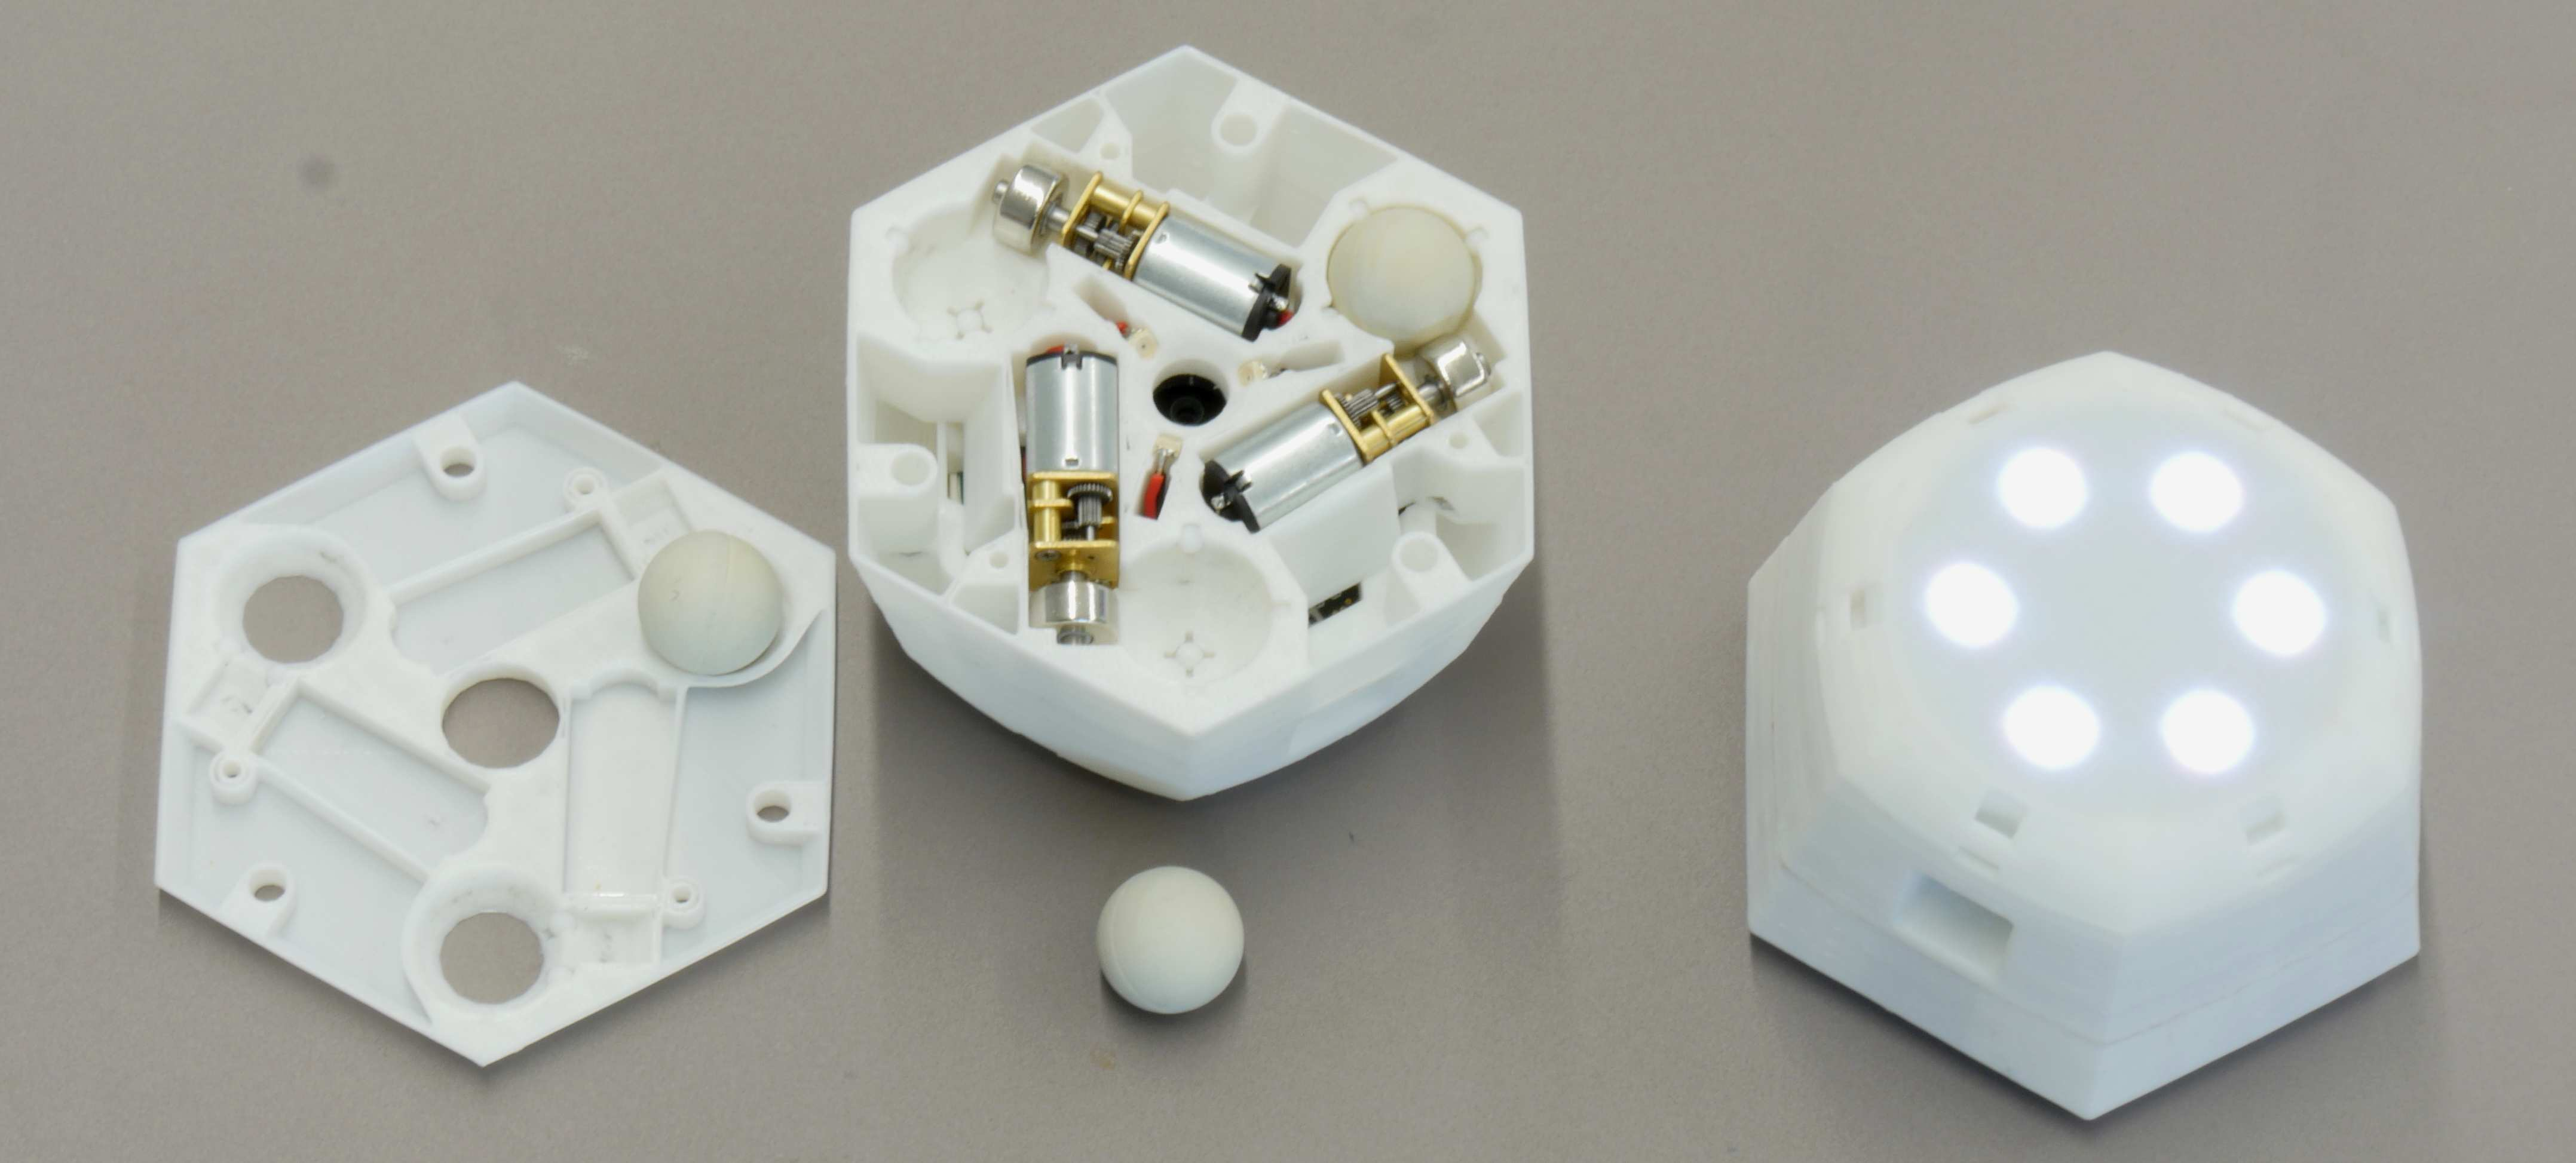
\includegraphics[height=6cm]{cellulo.jpg}
    \caption{Cellulo}
    \label{fig:Cellulo}
\end{figure}
  
\begin{figure}[htbp]
    \centering
    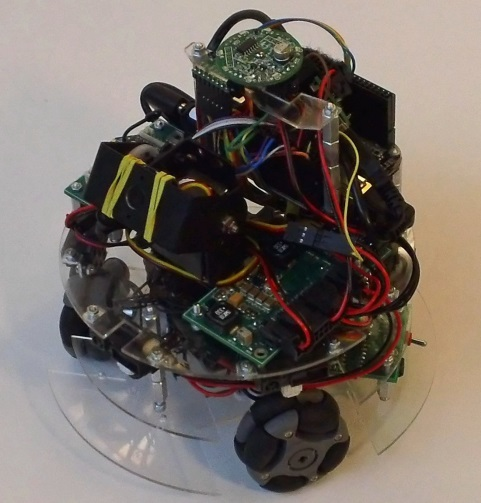
\includegraphics[height=10cm]{WolfBot.jpg}
    \caption{WolfBot}
    \label{fig:WolfBot}
\end{figure}

经过尝试,我们发现磁驱电机的速度和磁环的磁性强弱、电池的电量剩余、磁环和轴之间的胶合强度等不可控因素关系很大,无法建立起小车各轮速度和电机PWM占空比之间的时不变映射关系,导致很难控制小车的走向和速度,最终放弃了这一想法。

WolfBot采用的全向轮和电机直接连接,使得底盘占地面积很大。最终我们则采用1.5英寸麦克纳姆轮(如图~\ref{fig:Wheel})和GW12-N20减速电机(如图~\ref{fig:GM12})(减速齿轮中的蜗杆改变90度传动方向)实现系统最小化。

\begin{figure}
    \begin{minipage}{0.48\textwidth}
      \centering
      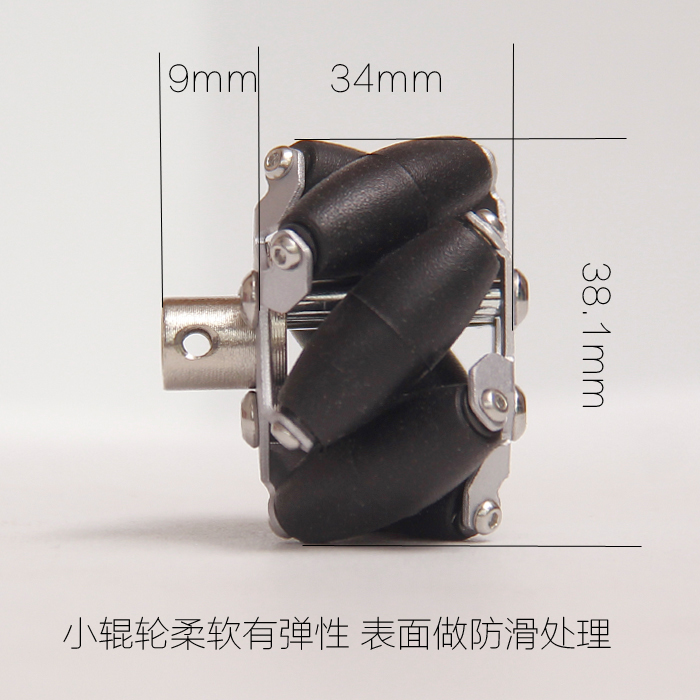
\includegraphics[height=5cm]{Wheel.jpg}
      \caption{使用的1.5英寸麦克纳姆轮}
      \label{fig:Wheel}
    \end{minipage}\hfill
    \begin{minipage}{0.48\textwidth}
      \centering
      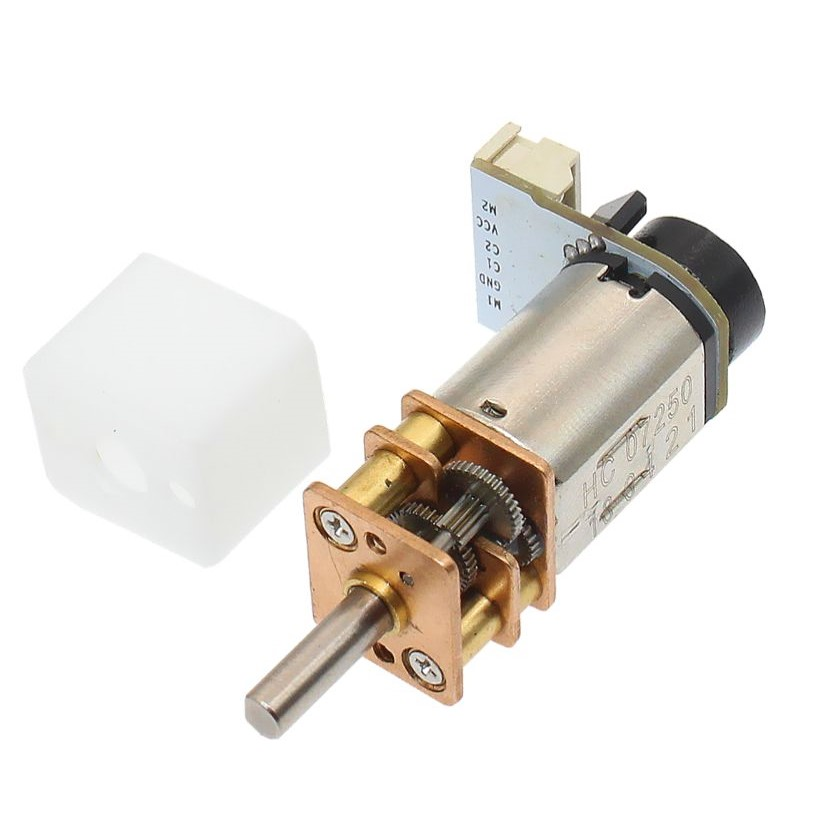
\includegraphics[height=5cm]{CHF-GM12-N20V.jpg}
      \caption{GW12-N20减速电机}
      \label{fig:GM12}
    \end{minipage}
\end{figure}

\section{三轮全向轮移动平台}
全向轮与麦克纳姆轮的共同点在于他们都由两大部分组成:轮毂和辊子(roller)。轮毂是整个轮子的主体支架,辊子则是安装在轮毂上的鼓状物。全向轮的轮毂轴与辊子转轴相互垂直,而麦克纳姆轮的轮毂轴与辊子转轴呈 45° 角。

经典的三轮全向轮(Omni Wheel)平台的全向轮中心平均分布在一个圆上。

\begin{equation}
    \left[\begin{array}{l}
    {V_{1}} \\
    {V_{2}} \\
    {V_{3}}
    \end{array}\right]=\left[\begin{array}{ccc}
    {-1} & {0} & {L} \\
    {\sin \frac{\pi}{6}} & {-\cos \frac{\pi}{6}} & {L} \\
    {\sin \frac{\pi}{6}} & {\cos \frac{\pi}{6}} & {L}
    \end{array}\right]\left[\begin{array}{l}
    {V_{x}} \\
    {V_{y}} \\
    {\omega}
    \end{array}\right]
\end{equation}

解算可得V1、V2、V3表达式:

\begin{equation}
    \left\{\begin{aligned}
    &V_{1}=-\frac{1}{2} V_{x}+\frac{\sqrt{3}}{2} V_{y}+L \omega \\
    &V_{2}=-\frac{1}{2} V_{x}-\frac{\sqrt{3}}{2} V_{y}+L \omega \\
    &V_{3}=V_{x}+L \omega
    \end{aligned}\right.
\end{equation}

\section{麦克纳姆轮}

\subsection{Mecanum wheel简介}
当需要车辆全向运动时,可以使用麦克纳姆轮(Mecanum wheel),如图~\ref{fig:Mecanum-wheel}。车辆可以沿着规定的路径移动,并同时绕其中心任意旋转,如图~\ref{fig:Vehicle-with-3-Mecanum-wheels}。麦克纳努姆轮由围绕轮轴排列的一组辊(roller)组成。

\begin{figure}
    \begin{minipage}{0.48\textwidth}
      \centering
      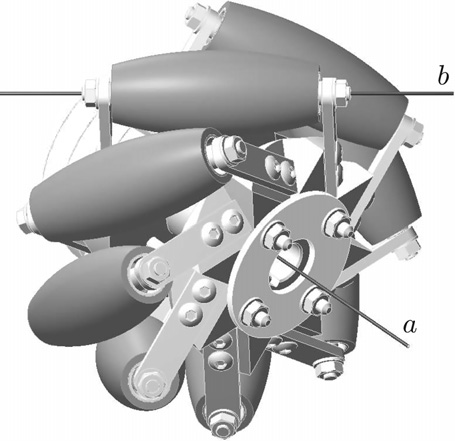
\includegraphics[height=5cm]{Mecanum-wheel.jpg}
      \caption{麦克纳姆轮}
      \label{fig:Mecanum-wheel}
    \end{minipage}\hfill
    \begin{minipage}{0.48\textwidth}
      \centering
      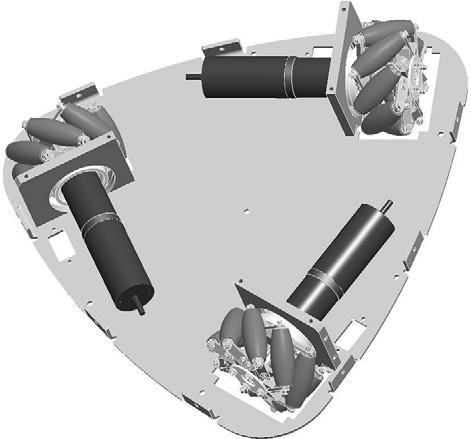
\includegraphics[height=5cm]{Vehicle-with-3-Mecanum-wheels.jpg}
      \caption{3麦克纳姆轮小车}
      \label{fig:Vehicle-with-3-Mecanum-wheels}
    \end{minipage}
\end{figure}

\subsection{Mecanum wheel几何描述}
为了使麦克纳姆轮能够在任意时刻都至少有一个辊子紧密接触地面,其几何学描述见图~\ref{fig:Curve-cR-generating-the-rolls}和图~\ref{fig:The-roll-surface-R},推导见Geometry and kinematics of the Mecanum wheel\cite{gfrerrer2008geometry}一文。

\begin{figure}[htbp]
    \centering
    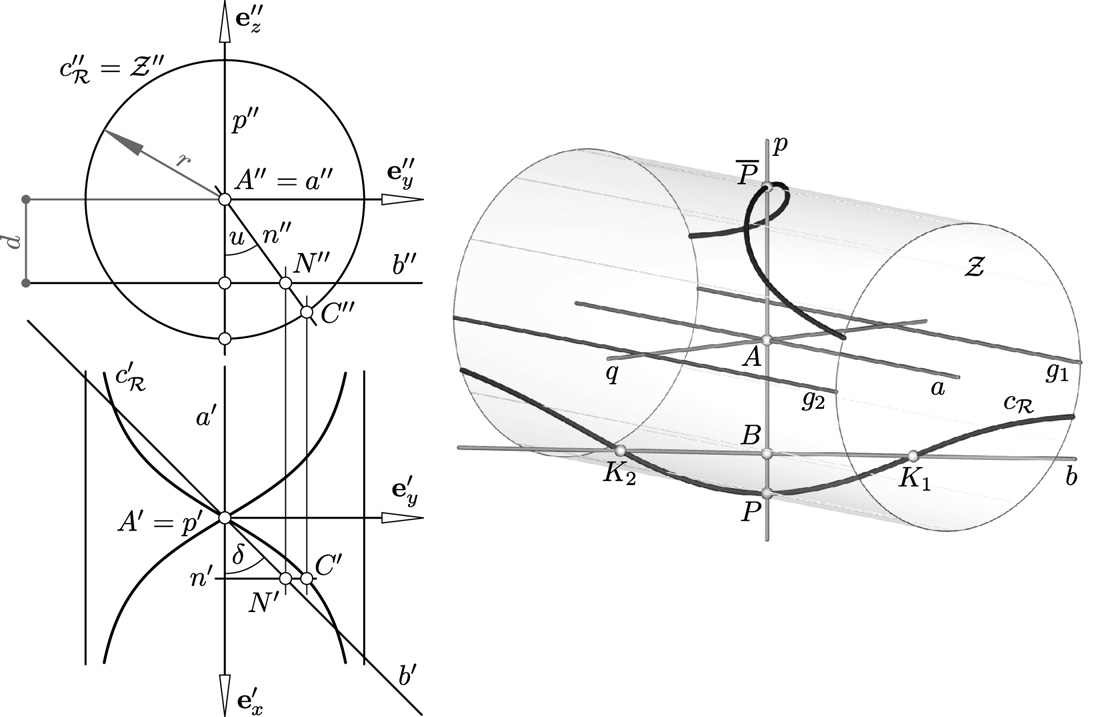
\includegraphics[height=10cm]{Curve-cR-generating-the-rolls.jpg}
    \caption{生成辊子曲面的曲线cR}
    \label{fig:Curve-cR-generating-the-rolls}
\end{figure}

\begin{figure}[htbp]
    \centering
    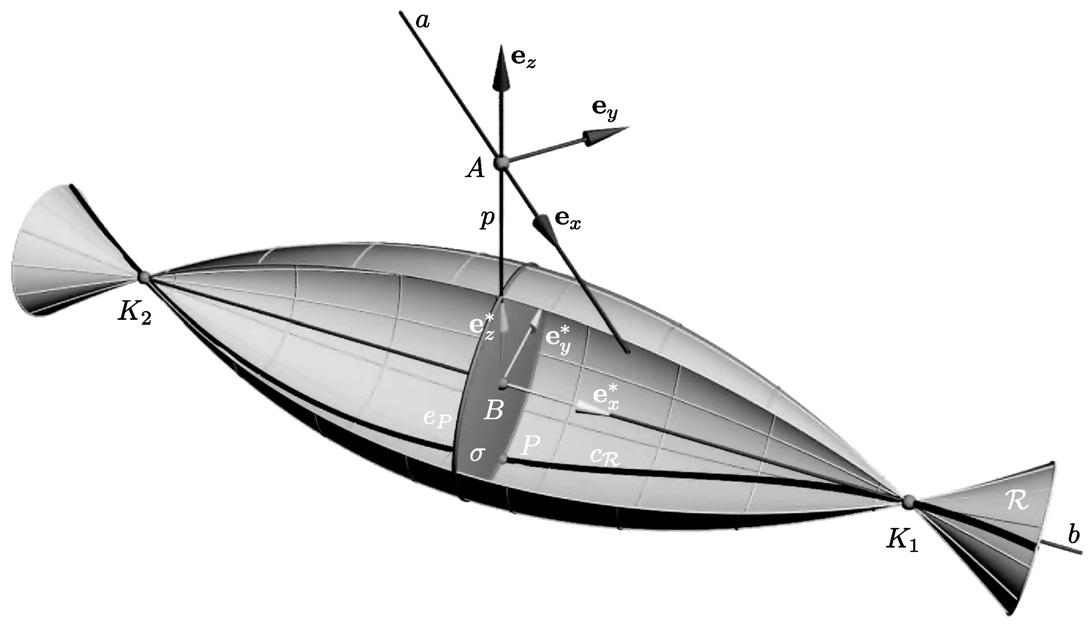
\includegraphics[height=8cm]{The-roll-surface-R.jpg}
    \caption{辊子曲面R}
    \label{fig:The-roll-surface-R}
\end{figure}

\subsection{Mecanum wheel动力学模型}

考虑一种装有麦克纳姆轮的车辆在水平地面上行驶,如图~\ref{fig:Vehicle-with-3-Mecanum-wheels}所示。分析某一时刻t(如图~\ref{fig:Velocities-Mecanum})上一个车轮的情况。

\begin{figure}[htbp]
    \centering
    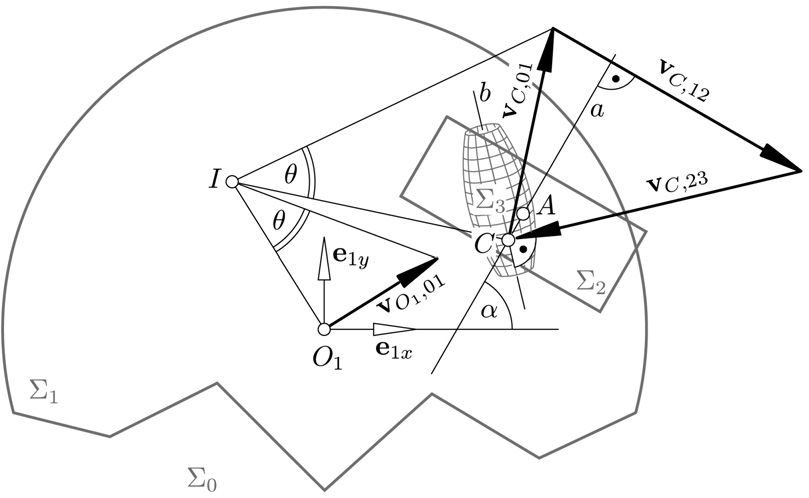
\includegraphics[height=10cm]{Velocities-Mecanum.jpg}
    \caption{麦克纳姆轮小车速度计算}
    \label{fig:Velocities-Mecanum}
\end{figure}

涉及四个系统:地面$\Sigma_{0}$,车$\Sigma_{1}$,车轮$\Sigma_{2}$和辊子$\Sigma_{3}$,这时在点C(接触点)接触地面。注意,该点始终位于车轮$\Sigma_{2}$的轴a之下:它是车轮转轴a和辊子转轴b在$\Sigma_{0}$中的正交投影的交点。仅在b处于水平位置的情况下,C才位于车轮中心A下方!

为了进行分析描述,我们选择$\Sigma_{1}$中的任意点$O_{1}$(“车辆中心 vehicle center”)作为坐标系$S_{1}:=\left\{O_{1} ; \mathbf{e}_{1 x}, \mathbf{e}_{1 y}, \mathbf{e}_{1 z}\right\}$的原点,与$\Sigma_{1}$相切,x和y轴平行于地面。车轮中心A可能有x和y坐标$a_x$和$a_y$。考虑到$S_1$和α可以表示$\mathbf{e}_{1 x}$与车轮轴线a之间的角度,则:

\begin{equation}
    \mathbf{a}=\left(\begin{array}{c}
    {\cos \alpha} \\
    {\sin \alpha} \\
    {0}
    \end{array}\right)
\end{equation}

是a轴的方向向量,辊子转轴的方向向量b取决于车轮的旋转角度u:

\begin{equation}
    \mathbf{b}=\left(\begin{array}{c}
    {\cos \alpha \cos \delta-\sin \alpha \sin \delta \cos u} \\
    {\sin \alpha \cos \delta+\cos \alpha \sin \delta \cos u} \\
    {\sin \delta \sin u}
    \end{array}\right)=:\left(\begin{array}{l}
    {b_{x}} \\
    {b_{y}} \\
    {b_{z}}
    \end{array}\right)
\end{equation}

在$S_1$坐标系中,接触点C的x和y坐标为:

\begin{equation}
    \left.\begin{array}{l}
    {c_{x}=a_{x}-d \cos \alpha \cot \delta \tan u} \\
    {c_{y}=a_{y}-d \sin \alpha \cot \delta \tan u}
    \end{array}\right\}
\end{equation}


在以下考虑中,我们可以忽略$z$-轴,因为出现的速度矢量都与$x y$平面平行。

在$t$时刻,令 $\omega$ 为 $\Sigma_{1} / \Sigma_{0}$ (vehicle/ground)运动的速度向量,$\mathbf{v}_{O_{1}, 01}=\left(v_{x}, v_{y}\right)^{\top}$ 为 $O_{1}$ 的速度向量。对于$\Sigma_{1} / \Sigma_{0}$相对运动,接触点C的速度向量为:

\begin{equation}
\mathbf{v}_{C, 01}=\left(\begin{array}{c}
{v_{x}-\omega c_{y}} \\
{v_{y}+\omega c_{x}}
\end{array}\right)
\end{equation}

$\Sigma_{2} / \Sigma_{1}$ (wheel/vehicle) 相对运动是绕轴a的简单旋转,因此,该相对运动C的速度矢量为


\begin{equation}
    \mathbf{v}_{C, 12}=\dot{u} r\left(\begin{array}{c}
    {-\sin \alpha} \\
    {\cos \alpha}
    \end{array}\right)
\end{equation}

其中 $\dot{u}=\frac{d u}{d t}$ 是 $\Sigma_{2} / \Sigma_{1}$ 的角速度。

$\Sigma_{3} / \Sigma_{2}$ (roll/wheel) 是绕$b$的旋转,因此,$C$的瞬时矢量速度 $\mathbf{v}_{\mathrm{C}, 23}$ 是垂直于 $\mathbf{b}$ 的:

\begin{equation}
\mathbf{v}_{C, 23}=\lambda\left(\begin{array}{c}
{-b_{y}} \\
{b_{x}}
\end{array}\right)
\end{equation}

因为辊子(被动)在地面上不滑动,$\Sigma_{3} / \Sigma_{0}$(roll/ground)的C速度$\mathbf{v}_{\mathrm{C}, 03}$必须为零。根据速度叠加原理,我们得到:

\begin{equation}
    \mathbf{v}_{C, 01}+\mathbf{v}_{C, 12}+\mathbf{v}_{C, 23}=\mathbf{v}_{C, 03}=\mathbf{o}=(0,0)^{\top}
\end{equation}

综上:

\begin{equation}
    \left.\begin{array}{l}
    {r \sin \alpha \dot{u}+b_{y} \lambda=v_{x}-\omega c_{y}} \\
    {r \cos \alpha \dot{u}+b_{x} \lambda=-v_{y}-\omega c_{x}}
    \end{array}\right\}
\end{equation}

通过消去λ得到微分方程:

\begin{equation}
    r\left(b_{x} \sin \alpha-b_{y} \cos \alpha\right) \dot{u}-b_{x}\left(v_{x}-\omega c_{y}\right)-b_{y}\left(v_{y}+\omega c_{x}\right)=0
\end{equation}

代入经简化的初始条件 $b_{x}=\cos (\alpha+\delta), b_{y}=\sin (\alpha+\delta), c_{x}=a_{x}, c_{y}=a_{y}$ 得:

\begin{equation}
    \label{eq:u}
    \dot{u}=-\frac{1}{r \sin \delta}\left[\sin (\alpha+\delta)\left(v_{y}+\omega a_{x}\right)+\cos (\alpha+\delta)\left(v_{x}-\omega a_{y}\right)\right]
\end{equation}

给定车速数据 $v_{x}, v_{y}, \omega$,该公式可以计算(近似)车轮转速$\dot{u}$。

\subsection{三麦克纳姆轮系统运动控制}

研究一个装有三个Mecanum轮,车轮中心为$A_{i}\left(a_{i x}, a_{i y}\right)$,主动轮轮轴角$\alpha_{i}, i=1,2,3$,子轮角度是$\delta$的小车,如果我们用$\omega_i$表示每个车轮的角速度,则根据等式~\ref{eq:u}我们有:

\begin{equation}
    \label{eq:inverse}
    \left(\begin{array}{l}
    {\omega_{1}} \\
    {\omega_{2}} \\
    {\omega_{3}}
    \end{array}\right)=-\frac{1}{r \sin \delta} \mathbf{M}\left(\begin{array}{c}
    {v_{x}} \\
    {v_{y}} \\
    {\omega}
    \end{array}\right)
\end{equation}

其中:

\begin{equation}
    \mathbf{M}=\left(\begin{array}{ccc}
    {\cos \left(\alpha_{1}+\delta\right)} & {\sin \left(\alpha_{1}+\delta\right)} & {a_{1 x} \sin \left(\alpha_{1}+\delta\right)-a_{1 y} \cos \left(\alpha_{1}+\delta\right)} \\
    {\cos \left(\alpha_{2}+\delta\right)} & {\sin \left(\alpha_{2}+\delta\right)} & {a_{2 x} \sin \left(\alpha_{2}+\delta\right)-a_{2 y} \cos \left(\alpha_{2}+\delta\right)} \\
    {\cos \left(\alpha_{3}+\delta\right)} & {\sin \left(\alpha_{3}+\delta\right)} & {a_{3 x} \sin \left(\alpha_{3}+\delta\right)-a_{3 y} \cos \left(\alpha_{3}+\delta\right)}
    \end{array}\right)
\end{equation}

式~\ref{eq:inverse}是车辆逆运动学问题的解。

在本问题的情境下:

\begin{definition}
    逆运动学问题:给定小车速度和转动角速度,求三个轮子各自的转速。
\end{definition}

\begin{definition}
    正运动学问题:给定三个轮子各自的转速,求小车速度和转动角速度。
\end{definition}

显然,当且仅当$\operatorname{det} \mathbf{M} \neq 0$,正运动学问题存在唯一解

\begin{equation}
    \left(\begin{array}{c}
    {v_{x}} \\
    {v_{y}} \\
    {\omega}
    \end{array}\right)=-r \sin \delta \mathbf{M}^{-1}\left(\begin{array}{c}
    {\omega_{1}} \\
    {\omega_{2}} \\
    {\omega_{3}}
    \end{array}\right)
\end{equation}

\begin{theorem}\label{the:theorem1}
    The direct kinematics of a robot with three Mecanum wheels has a unique solution if and only if the wheels are arranged so that the roll axes are not concurrent or parallel.\hfill —— A. Gfrerrer
\end{theorem}

即:

\begin{theorem}\label{the:theorem1}
    当且仅当车轮排布使得小轮不平行时,3-Mecanum轮机器人才具有运动学唯一解。
\end{theorem}

\section{主控板}

\section{扩展接口}

\section{实物可视化界面}

\section{UI}